% Distributed Consensus Protocol TikZ Diagram
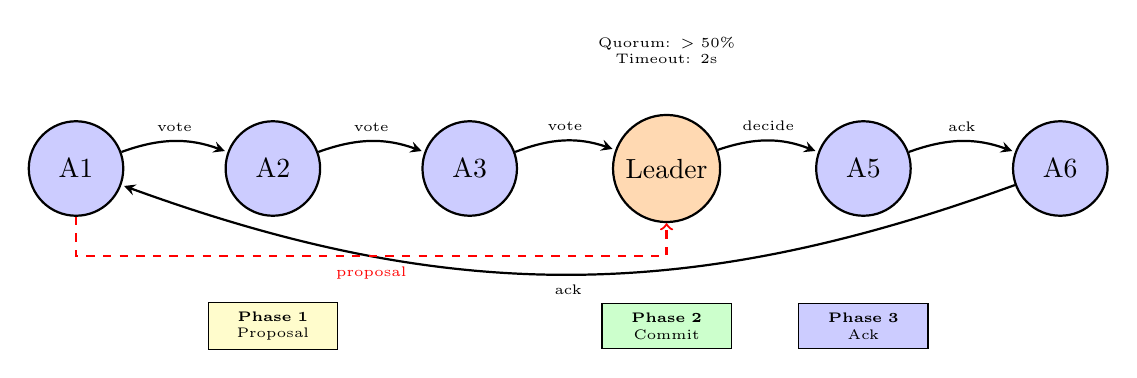
\begin{tikzpicture}[
    node distance=2cm,
    auto,
    agent/.style={
        circle,
        draw,
        fill=blue!20,
        thick,
        minimum size=1.2cm,
        align=center
    },
    leader/.style={
        circle,
        draw,
        fill=orange!30,
        thick,
        minimum size=1.3cm,
        align=center
    },
    arrow/.style={
        ->,
        thick,
        >=stealth,
        shorten >=1pt
    },
    label/.style={
        font=\footnotesize\itshape
    }
]

% Agents in ring
\node [agent] (a1) {A1};
\node [agent, right of=a1, node distance=2.5cm] (a2) {A2};
\node [agent, right of=a2, node distance=2.5cm] (a3) {A3};
\node [leader, right of=a3, node distance=2.5cm] (leader) {Leader};
\node [agent, right of=leader, node distance=2.5cm] (a5) {A5};
\node [agent, right of=a5, node distance=2.5cm] (a6) {A6};

% Ring connections
\draw [arrow] (a1) to[bend left=20] node[above, label, font=\tiny] {vote} (a2);
\draw [arrow] (a2) to[bend left=20] node[above, label, font=\tiny] {vote} (a3);
\draw [arrow] (a3) to[bend left=20] node[above, label, font=\tiny] {vote} (leader);
\draw [arrow] (leader) to[bend left=20] node[above, label, font=\tiny] {decide} (a5);
\draw [arrow] (a5) to[bend left=20] node[above, label, font=\tiny] {ack} (a6);
\draw [arrow] (a6) to[bend left=20] node[below, label, font=\tiny] {ack} (a1);

% Phases
\node [below of=a2, node distance=2cm, text width=4em, align=center, font=\tiny, fill=yellow!20, draw] {
    \textbf{Phase 1}\\
    Proposal
};

\node [below of=leader, node distance=2cm, text width=4em, align=center, font=\tiny, fill=green!20, draw] {
    \textbf{Phase 2}\\
    Commit
};

\node [below of=a5, node distance=2cm, text width=4em, align=center, font=\tiny, fill=blue!20, draw] {
    \textbf{Phase 3}\\
    Ack
};

% Quorum annotation
\node [above of=leader, node distance=1.5cm, text width=5em, align=center, font=\tiny] {
    Quorum: $>50\%$\\
    Timeout: 2s
};

% Message flow
\draw [dashed, ->, red, thick] (a1.south) -- ++(0,-0.5) -| node[near start, below, label, font=\tiny] {proposal} (leader.south);

\end{tikzpicture}
